47. \begin{figure}[ht!]
\center{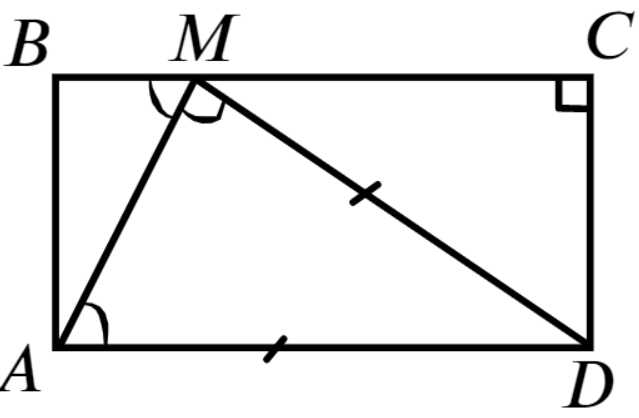
\includegraphics[scale=0.35]{g47.png}}
\end{figure}\\
Углы $BMA$ и $MAD$ являются накрест лежащими при параллельных прямых $BC$ и $AD,$ поэтому $\angle MAD=\angle BMA=\angle AMD$ (т.к. $MA$ --- биссектриса). Тогда в треугольнике $AMD$ равны углы при стороне $AM,$ значит он является равнобедренным и $MD=AD=2AB=2CD.$ Таким образом, в прямоугольном треугольнике $MCD$ катет $CD$ равен половине гипотенузы $MD,$ а значит он лежит напротив угла в $30^\circ,$ то есть $\angle DMC=30^\circ.$ Значит, $\angle BMA=(180^\circ-30^\circ):2=75^\circ.$\\
